\usetikzlibrary{shapes,positioning,arrows,calc}
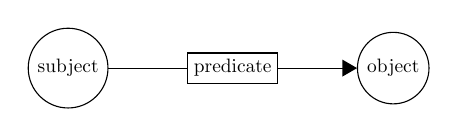
\begin{tikzpicture}[>= triangle 60,
  remember picture,
  every node/.style={scale=0.7},
  ]
	\node [draw,circle] (subject) {subject} ;
	\node [draw,rectangle,right=of subject] (predicate) {predicate} ;
	\node [draw,circle,right=of predicate] (object) {object} ;
	\draw [->] (subject) -- (predicate) -- (object) ;
\end{tikzpicture}
